\documentclass[12pt, fleqn]{article}

\usepackage[left=0.75in, right=0.75in, bottom=0.75in, top=1.0in]{geometry}
\usepackage{amsmath}
\usepackage{amssymb}
\usepackage{amsthm}
\usepackage{mathtools}
\usepackage{hyperref}
\usepackage{ulem}
\usepackage{enumitem}
\usepackage{floatrow}
\usepackage{graphicx}
\usepackage[export]{adjustbox}
\usepackage{sectsty}
\renewcommand{\thesubsubsection}{(\alph{subsubsection})}

\usepackage[dvipsnames]{xcolor}
\usepackage[perpage]{footmisc}

\usepackage{fancyhdr}
\pagestyle{fancy}
\fancyhf{}
\lhead{190100044}
\rhead{Assignment 1}
\renewcommand{\footrulewidth}{1.0pt}
\cfoot{Page \thepage}

\setlength{\parindent}{0em}

\title{Assignment 1}
\author{Devansh Jain, 190100044}
\date{29 Aug 2021}

\newcommand{\twoxone}[2]{
    \begin{pmatrix}
        #1 \\
        #2
    \end{pmatrix}
}

\begin{document}

% \pagenumbering{gobble}
\maketitle
\tableofcontents
\thispagestyle{empty}
\setcounter{page}{0}

\newpage
\section{Ordinary Least Squares (OLS) Regression in one variable}

\subsection{CS337: Theory}
\begin{equation*}
  \begin{aligned}
    mse(w,b)                             & = \frac{1}{N} \sum_{i=1}^N ((w x_i + b) - y_i)^2                                                                                 \\
    \frac{\partial mse(w,b)}{\partial w} & = \frac{1}{N} \sum_{i=1}^N 2 \cdot ((w x_i + b) - y_i) \cdot x_i                                                                 \\
    \frac{\partial mse(w,b)}{\partial b} & = \frac{1}{N} \sum_{i=1}^N 2 \cdot ((w x_i + b) - y_i)                                                                           \\
    \nabla mse(w,b)                      & = \twoxone{\frac{\partial mse (w,b)}{\partial w}}{\frac{\partial mse (w,b)}{\partial b}}                                         \\
                                         & = \twoxone{\frac{1}{N} \sum_{i=1}^N 2 \cdot ((w x_i + b) - y_i) \cdot x_i}{\frac{1}{N} \sum_{i=1}^N 2 \cdot ((w x_i + b) - y_i)} \\
                                         & = \frac{2}{N} \twoxone{\sum_{i=1}^N ((w x_i + b) - y_i) \cdot x_i}{\sum_{i=1}^N ((w x_i + b) - y_i)}
  \end{aligned}
\end{equation*}

\subsection{CS335: Lab}
\subsubsection{}
Present in notebook

\subsubsection{}
Present in notebook

\subsubsection{}
\begin{figure}[H]
  \centering
  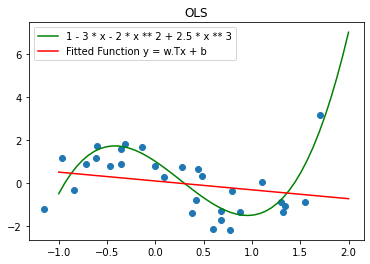
\includegraphics[scale=0.6]{singlevar_grad.png}
  \caption{Single Variable - Gradient Descent (epochs=1000)}
\end{figure}
\begin{figure}[H]
  \centering
  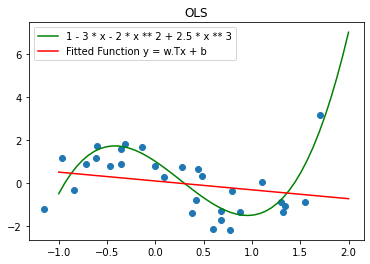
\includegraphics[scale=0.6]{singlevar_grad.png}
  \caption{Single Variable - Closed Form}
\end{figure}

\subsubsection{}
As mentioned in description of the question (point 5), the error function (mse) is convex and has just one minimum. \\
By using the closed form, we get the point corresponding to minimum mse error. As we compute the parameters based on training data, the training loss is minimum at this point. \\
Therefore, training loss for solution of \verb!singlevar_grad()! can never be strictly less than that of the solution obtained by \verb!singlevar_closedform()!.

\end{document}
